In the first prototypes, TRITIUM-IFIC-0 and TRITIUM-IFIC-1, the fibers were directly coupled to the photosensor, so the detected photons were only those guided by the fibers. However, in the last prototypes, TRITIUM-Aveiro and TRITIUM-IFIC-2, two PMMA windows are used, which allows the transmission to the photosensors of the photons guided by the fiber and photons that propagate through the water at the cost of losing some photons when passing through the PMMA (approximately $5\%$ at the working wavelength, experimentally measured in Figure \ref{fig:PMMATransmissionSpectrum}). To quantify the importance of the latter contribution, the TRITIUM-Aveiro prototype was simulated. The distribution of the number of photons that reach the PMMA per tritium event is shown in Figure \ref{fig:PMMAEffect}. Fiber-guided photons are shown in a red distribution, while those traveling in the water medium are plotted in the blue histogram. It can be seen that the tritium signal obtained from the water is as important as that obtained from the fibers. Therefore, the use of PMMA windows improve the tritium detection efficiency by a factor of almost 2.

\begin{figure}[hbtp]
\centering
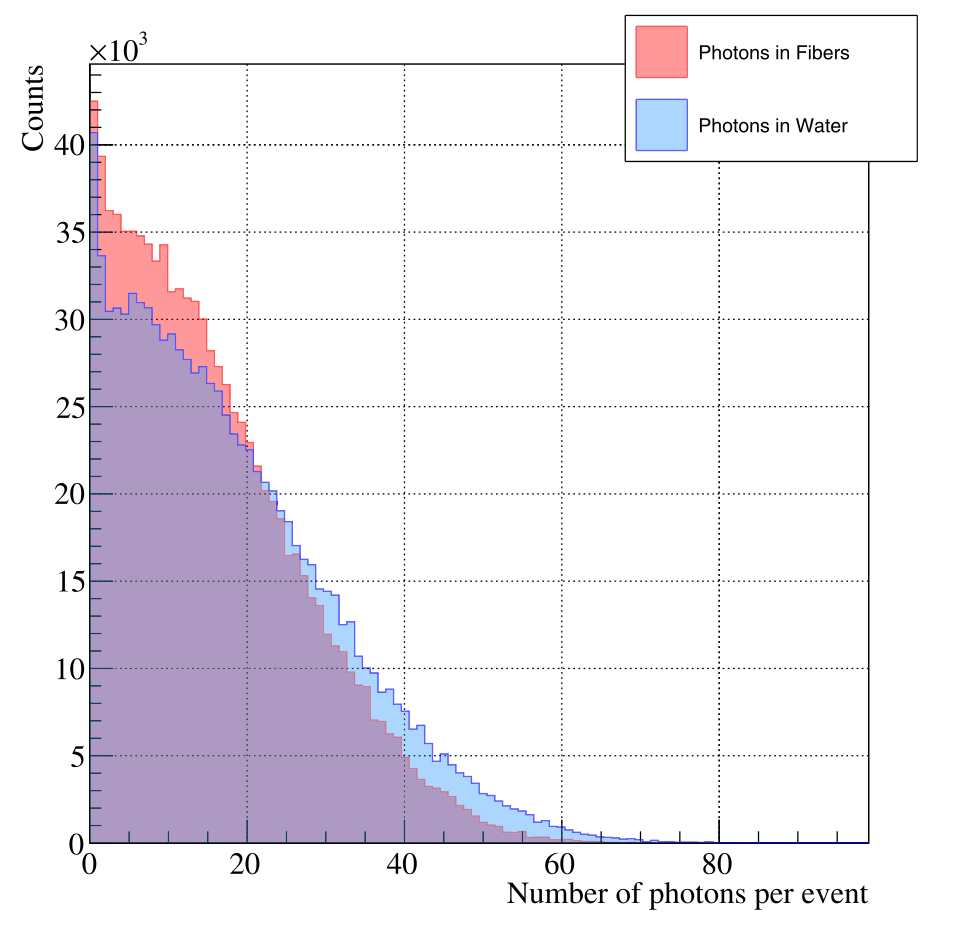
\includegraphics[scale=0.3]{Figures/8SimulationsResults/81TRITIUMDesign/815PMMA/PhotonsDetectedWaterFiber.png}
\caption{Distribution of photons reaching the PMMA windows. The red histogram corresponds to the photons guided by fibers and the blue histogram to photons traveling in the water \cite{SimulationPaperCarlos}.\label{fig:PMMAEffect}}
\end{figure}

